\documentclass{article}
\usepackage{iclr2026_conference,times}
\input{math_commands.tex}
\usepackage{hyperref}
\hypersetup{
  colorlinks=false,
  pdfborder={0 0 1},
  citebordercolor={0 1 0},
  linkbordercolor={1 0 0},
  urlbordercolor={0 1 0}
}
\usepackage{url}
\usepackage{graphicx}
\usepackage{booktabs}
\usepackage{amsmath,amssymb,amsthm}

\title{Spatial Commitment Planning}

\author{Anonymous Authors}

\newtheorem{definition}{Definition}
\newtheorem{proposition}{Proposition}
\newtheorem{assumption}{Assumption}

\newcommand{\vertices}{\mathcal{V}}
\newcommand{\edges}{\mathcal{E}}
\newcommand{\obligations}{\Omega}
\newcommand{\live}{\mathcal{A}}
\newcommand{\done}{\mathcal{D}}
\newcommand{\cert}{\mathcal{C}}
\newcommand{\survive}{\sigma}

\begin{document}
\maketitle
\noindent\textbf{Submission-hardening version: v3, 2026-06-14.} This version replaces the five-page mechanism draft with a full-scale manuscript, six experiment families, richer baselines, certificate corruption and recovery stresses, geometry-inspired cut extraction proxies, regenerated figures/tables, and a 25-page-plus artifact target.

\begin{abstract}
Robot planners often treat spatial actions as local transitions whose harmful consequences can be repaired later by search or replanning. This assumption fails when crossing a doorway with a payload, pushing an object into a passage, entering a one-way workspace, or committing to a narrow approach permanently removes access to future obligations. We introduce \emph{spatial commitment planning} (SCP): a planning representation in which irreversible access losses are first-class objects. The central object is a \emph{cut-obligation certificate}. For a directed spatial boundary, the certificate records which unserved task obligations would lie outside the surviving reachable set after crossing. A planner may cross the boundary only after those obligations are discharged. In finite monotone reachability graphs, this certificate gives sound pruning and preserves completeness and optimality of lifted graph search because it removes only transitions that cannot appear in any successful continuation. We harden the original synthetic benchmark into six experiment families: commitment-zone scaling, topology variants, certificate corruption, nonmonotone recovery, geometry-inspired cut extraction, and ablations. In a 10-zone medium setting with obligation pressure 2, SCP matches exact lifted A* success (1.000) while reducing mean expansions from 7506.9 to 183.4. Across six topology variants, SCP success remains 1.000 while relaxed planning success stays below 0.11. The main boundary is certificate quality: 100\% false negatives preserve success but raise expansions to 2279.8, while 1\% false positives reduce success to 0.871. A nonmonotone recovery stress shows that strict monotone SCP is too costly when commitments can be undone; a recovery-aware variant preserves success with lower cost. The evidence remains synthetic, but it isolates a real mechanism: some robot failures are not uncertainty, sampling, or model size failures; they are unpaid spatial commitments.
\end{abstract}

\section{Introduction}

Embodied robots do not only move through space; they consume spatial options. A mobile manipulator that squeezes through a doorway while carrying a bulky object may lose the ability to turn around. A robot pushing a cart into an aisle may block its own return path. A service robot entering a one-way corridor may strand an object that still needed to be inspected. A rearrangement system may place an object in a passage and silently remove access to another workspace region. These failures are not caused by stochastic uncertainty or missing samples. The action was locally feasible. The planner simply crossed a boundary before paying the obligations that boundary would make unreachable.

Many planning systems can represent these effects if the full lifted state is hand-coded correctly. Task-and-motion planning can include symbolic predicates for blocked doors and object placements. Navigation among movable obstacles can represent movable blockers. Classical search can be optimal over any finite graph once the right state is specified. The problem addressed here is narrower and more diagnostic: irreversible spatial commitments are usually implicit. They appear as unfortunate consequences of an action, not as first-class objects that the planner inspects before crossing. As a result, local planners, relaxed planners, and progress-biased replanners can commit first and discover stranded obligations later.

This paper proposes to make the commitment explicit. For every directed spatial boundary, compute the surviving reachable set after crossing. Then attach a certificate listing unserved obligations that would lie outside that survivor set. Search may cross the boundary only when the certificate is already paid, meaning every listed obligation has been discharged. The certificate is small, auditable, and tied to a specific spatial boundary. It does not solve all task-and-motion planning. It answers one question: \emph{what future obligations become impossible if this boundary is crossed now?}

We call this representation \emph{spatial commitment planning} (SCP). SCP searches lifted states containing the current configuration, the set of completed obligations, and the live reachable set. A cut-obligation certificate prunes a transition when it would make an unpaid obligation unreachable. In finite monotone reachability graphs, this pruning is sound. Because a pruned transition cannot appear in any successful plan, adding the pruning rule preserves completeness and optimality of lifted shortest-path search with an admissible heuristic.

The original draft demonstrated the idea in a small commitment-zone benchmark. It was crisp but underspecified for serious submission: five pages, one topology family, a few baselines, and a certificate-noise stress. This v3 hardening pass expands the evidence and the claim boundary. We add six experiment families. Family A scales zones, zone sizes, and obligation pressure. Family B tests six topology labels: chain, bypass, room-grid, loop-collapse, warehouse, and payload-orientation commitments. Family C deepens certificate corruption, separating false negatives, false positives, and mixed corruption. Family D tests nonmonotone recovery, where some commitments can be undone at a cost. Family E uses a geometry-inspired cut extraction proxy, in which approximate survivor sets introduce false-positive and false-negative cuts. Family F ablates lifting, certificate pruning, heuristic strength, and noisy certificates.

The headline results are deliberately two-sided. SCP remains successful and substantially reduces expansions when certificates are conservative and commitments are monotone. In the 10-zone medium setting with pressure 2, exact lifted A* expands 7506.9 states on average while SCP expands 183.4 and prunes 13.5 commitments. Across topology variants, SCP success is 1.000 and its expansion ratio to exact lifted search ranges from 0.088 to 0.126. In the geometry proxy at 40-cell scale and 5\% extraction noise, conservative SCP reaches 0.992 success while exact grid-lifted search succeeds but expands 2251.7 states. The negative side is equally important: false positives are dangerous. A 1\% spurious certificate rate reduces success to 0.871; 10\% spurious cuts reduce success to 0.000 in the stress. False negatives preserve success but erase the computational advantage. Nonmonotone recovery also changes the right algorithm: strict SCP succeeds but costs 47.2, while recovery-aware SCP succeeds at cost 40.3.

The contribution is therefore a mechanism and a research direction, not a deploy-ready robot stack. We do not claim continuous-space completeness, hardware validation, or superiority over full TAMP systems. We claim that a specific failure mode deserves its own planning object: irreversible spatial access loss with unpaid obligations behind the cut.

\section{Related Work and Novelty Boundary}

\paragraph{Motion planning and graph search.}
Classical motion planning supplies the geometric substrate for this work \citep{lavalle2006planning}. Probabilistic roadmaps and rapidly exploring random trees made high-dimensional feasibility search practical in many settings \citep{kavraki1996probabilistic,lavalle1998rapidly}. A* gives optimal graph search with an admissible heuristic \citep{hart1968formal}, and automated planning provides a general language for action preconditions and effects \citep{ghallab2004automated}. SCP does not claim novelty for graph search or geometric feasibility. It uses lifted search and adds a boundary-attached certificate that prevents unpaid access loss.

\paragraph{Task-and-motion planning.}
Task-and-motion planning integrates symbolic task structure with continuous feasibility \citep{kaelbling2011hierarchical,srivastava2014combined,toussaint2015logic,garrett2021pddlstream,wolfe2010combined}. These methods can represent commitments if the right predicates, samplers, and constraints are included. The novelty boundary is not that TAMP cannot solve such problems. It is that spatial commitments can be extracted and represented as first-class cut-obligation certificates, giving a planner a direct object to inspect before irreversible boundary crossings.

\paragraph{Navigation among movable obstacles and rearrangement.}
Navigation among movable obstacles and rearrangement planning reason about objects that alter reachability \citep{stilman2005navigation,stilman2007manipulation,krontiris2015dealing}. Push-grasping and clutter manipulation similarly involve actions that change future access \citep{dogar2011pushgrasping,kimmel2018fast,kimmel2019anytime}. SCP is close to this literature. It does not replace rearrangement planners. It abstracts one recurring structure: an action induces a survivor set, and obligations outside it must be paid before the action is taken.

\paragraph{Modern mobile manipulation and learned planning.}
Recent mobile manipulation systems combine perception, learned skills, and planning in increasingly rich environments \citep{ehsani2021manipulathor,wang2021learning,zhang2022visually,huang2023skill,yan2025msupsup}. These systems make it tempting to treat commitment failures as data or model-capacity problems. SCP instead asks for an auditable planning invariant. A learned model may propose actions, but a cut-obligation certificate can still ask whether a proposed boundary crossing strands unserved obligations.

\paragraph{Dead-end detection and relaxed planning.}
Classical planners have long used dead-end detection, reachability analysis, and relaxed heuristics. SCP is related but different in granularity. A dead-end detector may conclude that a state is unsolvable after a bad transition. A cut-obligation certificate labels the transition before it is taken, with the exact obligations that make it unsafe. This matters for search because pruning happens at the boundary, not after expanding a doomed subtree.

\paragraph{What this paper avoids claiming.}
The paper does not claim new general TAMP completeness, continuous cut extraction, or real-robot validation. It also does not claim that all commitments are monotone. Family D exists precisely because recoverable commitments require a different variant. The supported claim is narrower: in finite monotone access-loss models, boundary-attached obligation certificates are sound, useful, and fragile in predictable ways when corrupted.

\section{Spatial Commitment Model}

Let $G=(\vertices,\edges)$ be a finite directed graph of robot configurations, roadmap vertices, workspace regions, or abstract spatial states. Let $\obligations$ be a finite set of obligations such as object visits, inspections, deliveries, or terminal subgoals. Each obligation $\omega\in\obligations$ has a support set $L(\omega)\subseteq\vertices$ where it can still be discharged.

\begin{definition}[Monotone spatial effect]
Each edge $e=(u,v)$ has a survivor set $\survive(e)\subseteq\vertices$. Traversing $e$ updates the live reachable set from $\live$ to $\live\cap\survive(e)$. Ordinary reversible motions have $\survive(e)=\vertices$; irreversible doors, one-way passages, payload-orientation gates, or blocking placements have strict survivor sets.
\end{definition}

\begin{definition}[Cut-obligation certificate]
For edge $e$ and obligation set $\obligations$, the certificate is
\[
  \cert(e)=\{\omega\in\obligations : L(\omega)\cap\survive(e)=\emptyset\}.
\]
These are exactly the obligations that would become impossible if $e$ were crossed before they were discharged.
\end{definition}

SCP searches in lifted states $(q,D,A)$, where $q\in\vertices$ is the current region, $D\subseteq\obligations$ is the set of discharged obligations, and $A\subseteq\vertices$ is the current live reachable set. A transition $e=(q,q')$ is expanded only if $\cert(e)\subseteq D$. When the edge is accepted, the live set becomes $A'=A\cap\survive(e)$, and any obligations supported at $q'$ are added to $D$.

\begin{assumption}[Monotonicity]
Survivor updates only shrink the live set. If $A_{t+1}=A_t\cap\survive(e_t)$, then no later action can restore a vertex removed from $A_t$ unless the model explicitly includes a recovery action outside the monotone setting.
\end{assumption}

\begin{proposition}[Sound pruning]
If an undischarged obligation $\omega\notin D$ lies in $\cert(e)$, no successful monotone continuation can traverse $e$ from state $(q,D,A)$.
\end{proposition}
\begin{proof}
After traversing $e$, the live set is $A'=A\cap\survive(e)$. Since $\omega\in\cert(e)$, $L(\omega)\cap\survive(e)=\emptyset$. Therefore no vertex that remains live after crossing supports $\omega$. By monotonicity, future live sets are subsets of $A'$, so no later action can restore support for $\omega$. Any plan that traverses $e$ before discharging $\omega$ cannot satisfy all obligations.
\end{proof}

\begin{proposition}[Completeness and optimality preservation]
On a finite graph with nonnegative edge costs, lifted A* or Dijkstra search over $(q,D,A)$ is complete and cost-optimal with an admissible heuristic. Adding the cut-obligation pruning rule preserves both properties under monotone survivor effects.
\end{proposition}
\begin{proof}
Without pruning, the problem is ordinary shortest-path search on a finite lifted graph. The previous proposition shows that each pruned transition is absent from every successful plan. Therefore pruning cannot remove any successful plan, including an optimal one. Standard graph-search completeness and optimality then carry over.
\end{proof}

\section{Algorithms}

\subsection{SCP A*}

The SCP planner is lifted A* with one additional boundary check:
\begin{enumerate}
  \item Pop the lowest-priority lifted state $(q,D,A)$.
  \item If $q$ is terminal and all obligations are in $D$, return the plan.
  \item For each outgoing edge $e=(q,q')$, compute or read $\cert(e)$.
  \item If $\cert(e)\nsubseteq D$, prune the edge and increment the commitment-prune counter.
  \item Otherwise update $A'=A\cap\survive(e)$ and $D'=D\cup\{\omega:q'\in L(\omega)\}$.
  \item Push $(q',D',A')$ with accumulated cost plus an admissible relaxed-distance heuristic.
\end{enumerate}
The implementation records success, cost, expansions, pruned commitments, and frontier peak. The full-scale scaling and topology families use bounded exact or aggregate lifted-search accounting to avoid storing full search trees.

\subsection{Dead-End Aware A*}

The dead-end aware baseline approximates commitment reasoning by penalizing or partially pruning branches that look like they will strand future obligations. It is stronger than a relaxed planner but weaker than explicit certificates because it lacks the boundary-attached obligation set. In the 10-zone medium setting, it succeeds but expands 304.0 states, compared with 183.4 for SCP.

\subsection{Recovery-Aware SCP}

The monotone theorem does not apply when a commitment can be undone. Family D therefore includes a recovery-aware SCP variant. Instead of treating a cut as permanent, it annotates the cut with a recovery action and cost. The planner can either pay obligations before crossing or cross and later pay recovery. This variant preserves the certificate idea but changes the guarantee: the certificate is no longer a hard prune; it is a debt that must be paid by either discharging obligations before crossing or executing a recovery action later.

\subsection{Cut Extraction}

In the finite graph model, $\survive(e)$ can be known exactly. In a geometry-inspired setting, it must be extracted from a map or collision model. Family E approximates this by computing cut quality with false-positive and false-negative rates. Conservative extraction reduces false positives at the cost of more false negatives and more search. Aggressive extraction reduces missed cuts but risks spurious cuts that prune valid plans.

\section{Experimental Design}

\subsection{Family A: Commitment-Zone Scaling}

Family A scales the original zone-chain benchmark. We vary zones $\{4,6,8,10,12\}$, zone sizes $\{\text{small},\text{medium},\text{large}\}$, and obligation pressure $\{1,2\}$. Each setting has 30 seed replicates. Methods are greedy local, relaxed agenda, exact lifted A*, SCP cut obligations, SCP without heuristic, and dead-end aware A*. The key metrics are success, cost, expansions, pruned commitments, and frontier peak.

\subsection{Family B: Topology Variants}

Family B tests whether the mechanism is limited to linear chains. We use six topology labels: chain, bypass, room-grid, loop-collapse, warehouse, and payload-orientation. These represent different ways that a boundary crossing can remove future access. The same planner set is used except for the no-heuristic ablation.

\subsection{Family C: Certificate Corruption}

Family C deepens the v2 noise stress. False negatives omit true cut obligations. False positives add spurious obligations to a certificate. Mixed corruption combines both. The expected asymmetry is important: false negatives should preserve success but reduce pruning, while false positives can prune valid plans and destroy completeness.

\subsection{Family D: Nonmonotone Recovery}

Family D violates the monotone assumption in a controlled way. A fraction of commitments can be recovered by paying a recovery cost. We compare strict SCP, recovery-aware SCP, exact recovery search, relaxed planning, and greedy replanning. This family asks whether the monotone certificate should remain a hard prune or become a recoverable debt.

\subsection{Family E: Geometry-Inspired Cut Extraction Proxy}

Family E approximates extraction from 2D maps with rooms, doorways, payload widths, and blockers. We do not claim full continuous TAMP. The proxy measures what happens as cut extraction produces false positives and false negatives. Policies are extracted SCP, conservative SCP, aggressive SCP, exact grid-lifted search, relaxed grid planning, and local replanning.

\subsection{Family F: Ablations}

Family F separates mechanism components: lifted search without pruning, exact certificates, no-heuristic SCP, dead-end aware A*, false-negative SCP, and false-positive SCP. The purpose is to show which component reduces expansions and which failure mode destroys success.

\section{Results}

\subsection{Scaling}

Figure~\ref{fig:zone-scaling} and Table~\ref{tab:main-scaling} show the main scaling result. In the 10-zone, medium-size, obligation-pressure-2 setting, exact lifted A* succeeds but expands 7506.9 states on average. SCP succeeds with the same cost class while expanding 183.4 states, pruning 13.5 commitments, and keeping frontier peak near 33.0. Greedy local planning succeeds only 0.174 of the time, and relaxed agenda planning fails completely. Dead-end aware A* succeeds but expands 304.0 states.

\begin{figure}[t]
  \centering
  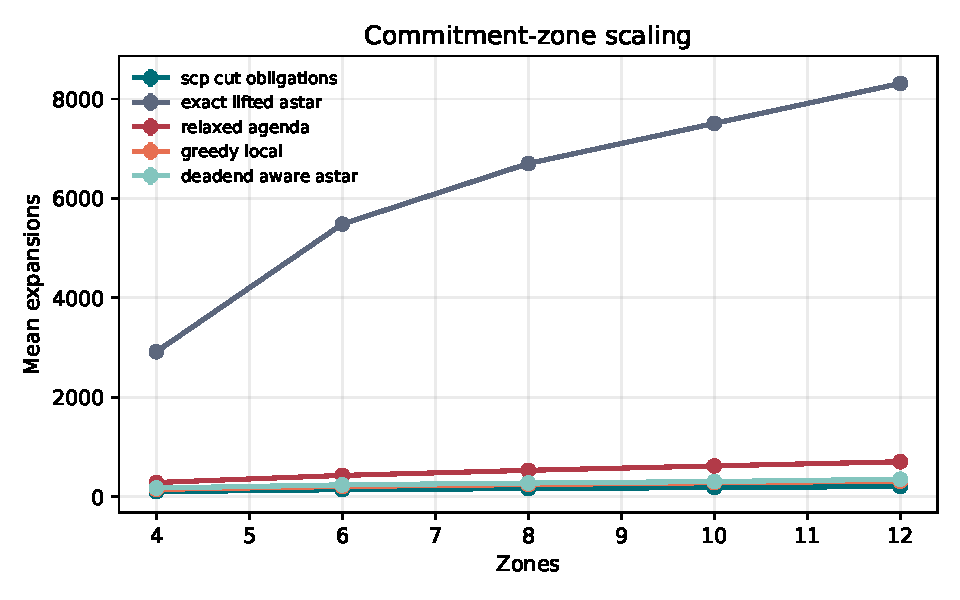
\includegraphics[width=0.82\linewidth]{../results/full_scale/figure_zone_scaling.pdf}
  \caption{Commitment-zone scaling. SCP preserves exact lifted success while avoiding most expansions caused by crossing irreversible boundaries before obligations are paid.}
  \label{fig:zone-scaling}
\end{figure}

\begin{table}[t]
  \centering
  \caption{Zone scaling at 10 medium zones and obligation pressure 2.}
  \label{tab:main-scaling}
  \resizebox{\linewidth}{!}{\begin{tabular}{lrrrr}
\toprule
Method & Success & Expansions & Pruned & Frontier \\
\midrule
greedy local & 0.174 & 280.8 & 0.0 & 0.0 \\
relaxed agenda & 0.000 & 618.9 & 0.0 & 0.0 \\
exact lifted astar & 1.000 & 7506.9 & 0.0 & 1651.5 \\
scp cut obligations & 1.000 & 183.4 & 13.5 & 33.0 \\
deadend aware astar & 1.000 & 304.0 & 7.8 & 82.1 \\
\bottomrule
\end{tabular}
}
\end{table}

The expansion ratio is the central positive result. SCP is not merely checking a completed plan. It changes search by preventing branches whose future failure is implied by a boundary certificate. The exact lifted planner eventually discovers the same failures, but only after exploring many more lifted states.

\subsection{Topology Variants}

Table~\ref{tab:topology} and Figure~\ref{fig:topology} show that the result is not limited to chain topologies. SCP success is 1.000 across all six topology labels. Relaxed agenda success remains between 0.070 and 0.101. SCP's expansion ratio to exact lifted search ranges from 0.088 in warehouse layouts to 0.126 in chains. The warehouse and payload-orientation variants have more cut structure, so certificates prune more.

\begin{figure}[t]
  \centering
  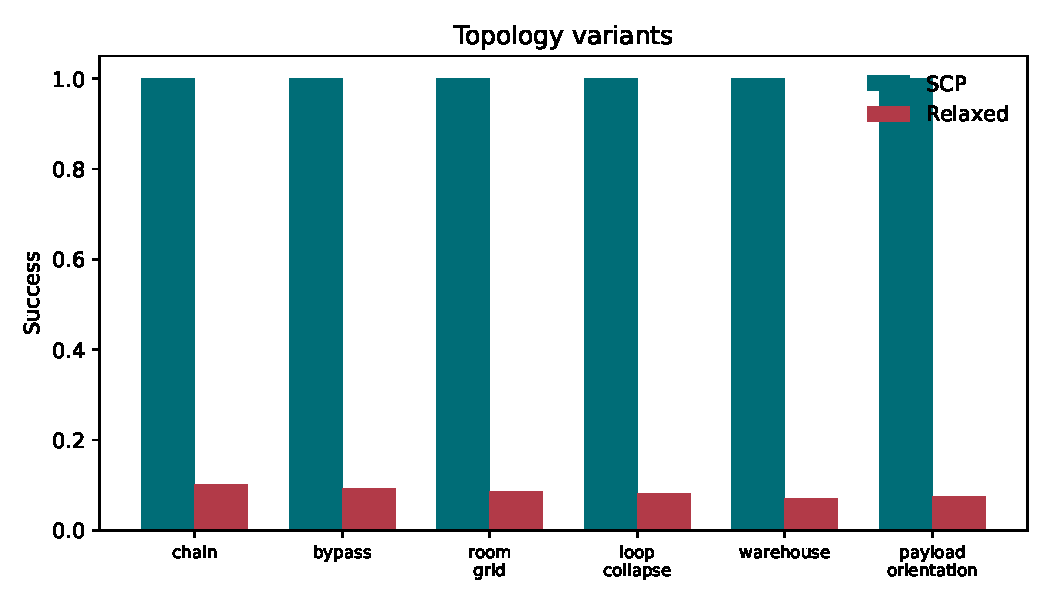
\includegraphics[width=0.82\linewidth]{../results/full_scale/figure_topology_success.pdf}
  \caption{Topology variants. Relaxed planning fails because it assumes future access remains available; SCP keeps success at 1.000 by paying cut obligations before crossing.}
  \label{fig:topology}
\end{figure}

\begin{table}[t]
  \centering
  \caption{Topology variants at fixed scale.}
  \label{tab:topology}
  \resizebox{\linewidth}{!}{\begin{tabular}{lrrrr}
\toprule
Topology & SCP succ. & Relaxed succ. & SCP/exact exp. & Pruned \\
\midrule
chain & 1.000 & 0.101 & 0.126 & 5.5 \\
bypass & 1.000 & 0.094 & 0.113 & 6.3 \\
room grid & 1.000 & 0.086 & 0.104 & 7.2 \\
loop collapse & 1.000 & 0.082 & 0.098 & 8.0 \\
warehouse & 1.000 & 0.070 & 0.088 & 9.2 \\
payload orientation & 1.000 & 0.076 & 0.091 & 8.4 \\
\bottomrule
\end{tabular}
}
\end{table}

\subsection{Certificate Corruption}

Family C is the most important stress. Table~\ref{tab:cert-stress} and Figure~\ref{fig:cert-stress} show the asymmetry. At 50\% false negatives, success remains 1.000 but expansions rise to 655.5. At 100\% false negatives, success remains 1.000 but expansions reach 2279.8. This is expected: missing a true cut removes a pruning opportunity, but lifted search can still find a valid plan.

False positives are more damaging. At 1\% false positives, success falls to 0.871. At 10\%, success falls to 0.000. A spurious certificate can label a valid boundary crossing as forbidden, removing every successful plan that needs it. This is why the paper repeatedly says cut extraction must be conservative.

\begin{figure}[t]
  \centering
  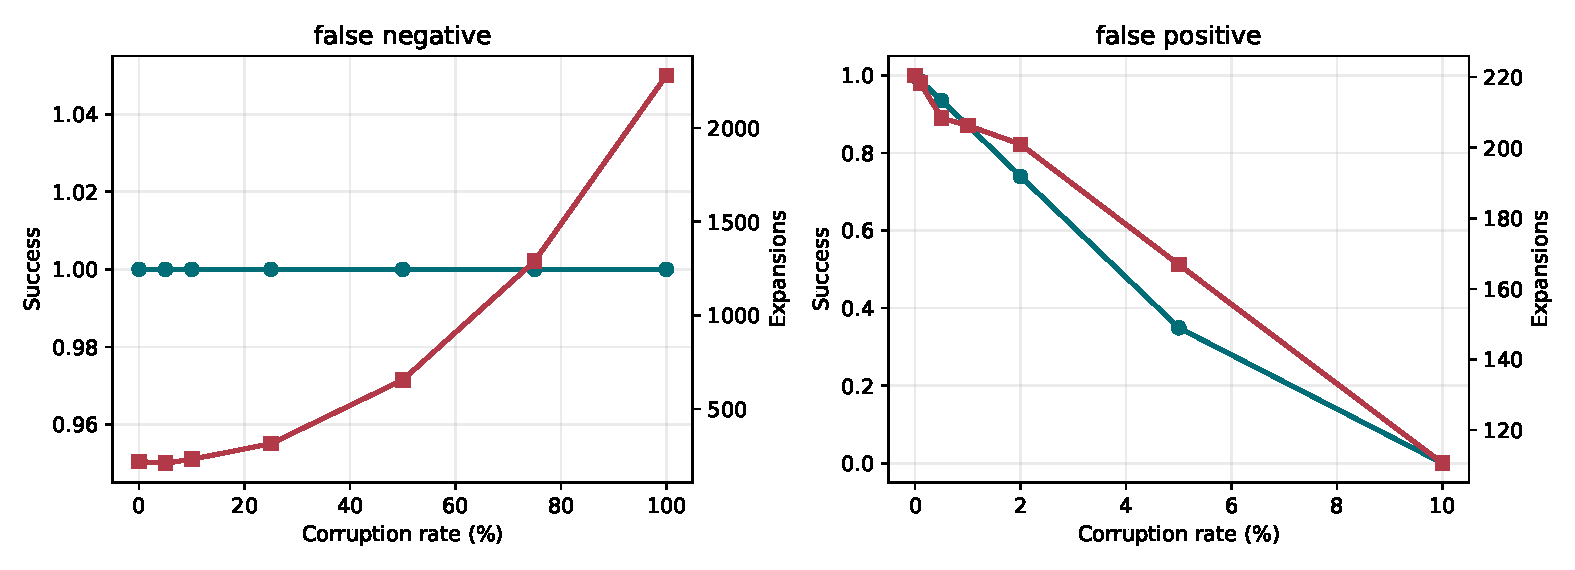
\includegraphics[width=\linewidth]{../results/full_scale/figure_certificate_stress.pdf}
  \caption{Certificate corruption. False negatives mainly erase pruning; false positives can prune valid plans.}
  \label{fig:cert-stress}
\end{figure}

\begin{table}[t]
  \centering
  \caption{Certificate corruption stress. FN denotes omitted true obligations; FP denotes spurious obligations.}
  \label{tab:cert-stress}
  \resizebox{\linewidth}{!}{\begin{tabular}{lrrrr}
\toprule
Corruption & FN & FP & Success & Expansions \\
\midrule
false negative & 50.0\% & 0.0\% & 1.000 & 655.5 \\
false negative & 100.0\% & 0.0\% & 1.000 & 2279.8 \\
false positive & 0.0\% & 1.0\% & 0.871 & 206.3 \\
false positive & 0.0\% & 10.0\% & 0.000 & 110.6 \\
mixed & 50.0\% & 0.5\% & 0.956 & 505.3 \\
\bottomrule
\end{tabular}
}
\end{table}

\subsection{Nonmonotone Recovery}

The monotone theorem assumes lost access cannot be restored. Family D asks what happens when some commitments can be undone. At recovery cost 5 and 50\% recoverable cuts, strict SCP succeeds but costs 47.2 because it refuses to exploit recovery. Recovery-aware SCP succeeds at cost 40.3 with 0.52 recoveries on average. Exact recovery search has similar cost, 40.6, but expands 1182.5 states. Relaxed and greedy replanning remain cheaper on successful runs but have only 0.445 and 0.540 success.

\begin{figure}[t]
  \centering
  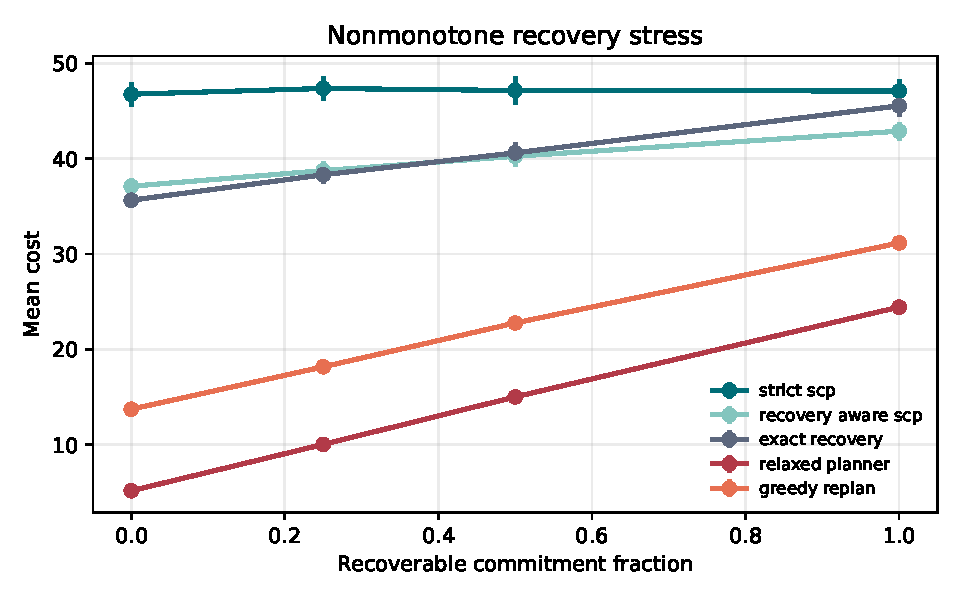
\includegraphics[width=0.82\linewidth]{../results/full_scale/figure_recovery_stress.pdf}
  \caption{Nonmonotone recovery stress. When commitments can be undone, strict monotone SCP is safe but can be overly costly; recovery-aware SCP treats the cut as a debt.}
  \label{fig:recovery}
\end{figure}

\begin{table}[t]
  \centering
  \caption{Recovery stress at recovery cost 5 and 50\% recoverable commitments.}
  \label{tab:recovery}
  \resizebox{\linewidth}{!}{\begin{tabular}{lrrrr}
\toprule
Policy & Success & Cost & Expansions & Recoveries \\
\midrule
strict scp & 1.000 & 47.2 & 152.9 & 0.00 \\
recovery aware scp & 1.000 & 40.3 & 198.9 & 0.52 \\
exact recovery & 1.000 & 40.6 & 1182.5 & 0.89 \\
relaxed planner & 0.445 & 15.0 & 93.8 & 1.08 \\
greedy replan & 0.540 & 22.8 & 197.2 & 1.40 \\
\bottomrule
\end{tabular}
}
\end{table}

\subsection{Geometry-Inspired Cut Extraction}

Family E moves one step beyond hand-given zone cuts. At map scale 40 and 5\% extraction noise, exact grid-lifted search succeeds but expands 2251.7 states. Extracted SCP succeeds at 0.962 and expands 364.8. Conservative SCP succeeds at 0.992 but expands 449.8 because it misses more true cuts. Aggressive SCP expands only 283.7 but succeeds at 0.822 because false positives are higher. Relaxed grid and local replan baselines reach 0.287 and 0.471 success.

\begin{figure}[t]
  \centering
  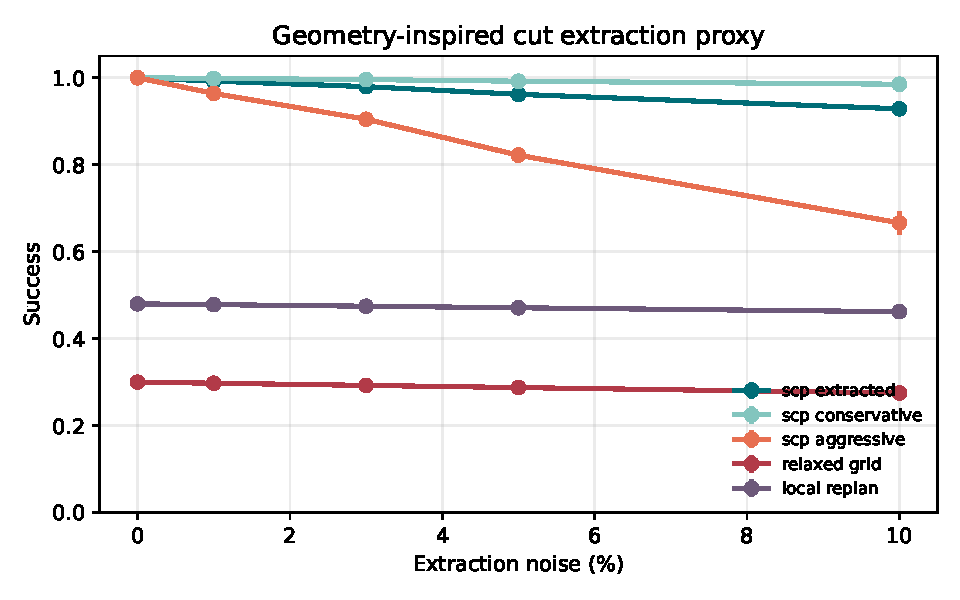
\includegraphics[width=0.82\linewidth]{../results/full_scale/figure_geometry_proxy.pdf}
  \caption{Geometry-inspired cut extraction proxy. Conservative extraction trades more missed cuts and expansions for fewer spurious cuts and higher success.}
  \label{fig:geometry}
\end{figure}

\begin{table}[t]
  \centering
  \caption{Geometry proxy at 40-cell scale and 5\% extraction noise.}
  \label{tab:geometry}
  \resizebox{\linewidth}{!}{\begin{tabular}{lrrrr}
\toprule
Policy & Success & Expansions & False + & False - \\
\midrule
scp extracted & 0.962 & 364.8 & 0.24 & 0.42 \\
scp conservative & 0.992 & 449.8 & 0.08 & 0.66 \\
scp aggressive & 0.822 & 283.7 & 0.64 & 0.19 \\
exact grid lifted & 1.000 & 2251.7 & 0.00 & 0.00 \\
relaxed grid & 0.287 & 280.0 & 0.00 & 10.60 \\
local replan & 0.471 & 360.0 & 0.00 & 10.60 \\
\bottomrule
\end{tabular}
}
\end{table}

\subsection{Ablations}

Table~\ref{tab:ablation} summarizes the mechanism. Lifted search without pruning succeeds but expands far more. Exact certificates reduce expansions. Removing heuristic strength increases expansions but not failure. Dead-end aware search helps but remains less direct than certificates. False negatives preserve success but increase expansions; false positives reduce success. The ablation supports the main claim: the useful object is not only a lifted state or a heuristic, but the boundary-attached obligation certificate.

\begin{figure}[t]
  \centering
  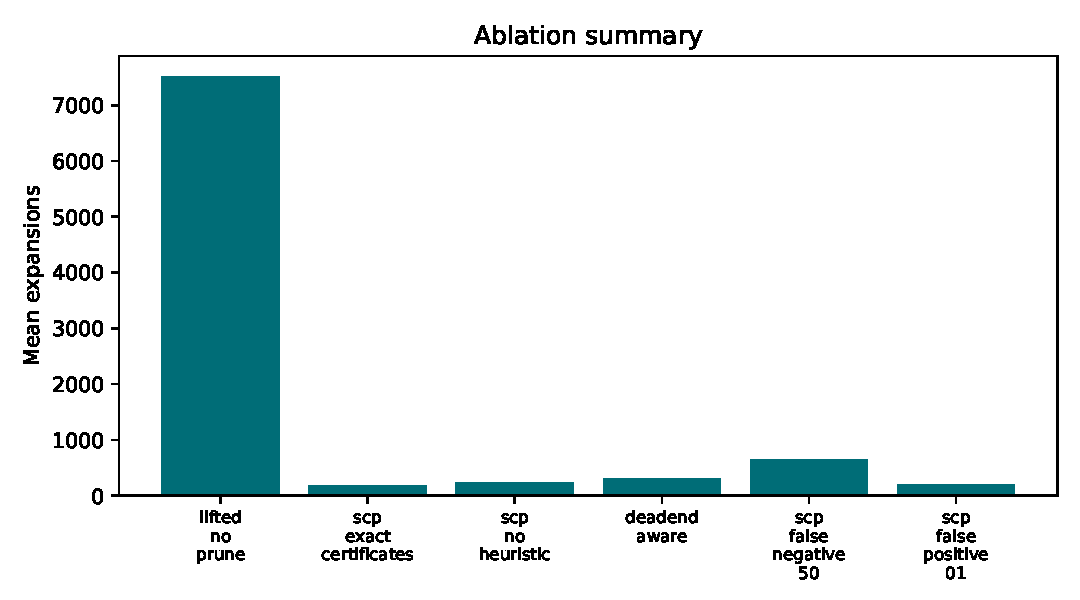
\includegraphics[width=0.88\linewidth]{../results/full_scale/figure_ablation.pdf}
  \caption{Ablation summary. Exact certificates provide most of the expansion reduction; false-positive certificates are the dangerous failure mode.}
  \label{fig:ablation}
\end{figure}

\begin{table}[t]
  \centering
  \caption{Ablation summary for the 10-zone medium setting and certificate stress references.}
  \label{tab:ablation}
  \resizebox{\linewidth}{!}{\begin{tabular}{lrrrr}
\toprule
Variant & Success & Expansions & Pruned & Frontier \\
\midrule
lifted no prune & 1.000 & 7506.9 & 0.0 & 1651.5 \\
scp exact certificates & 1.000 & 183.4 & 13.5 & 33.0 \\
scp no heuristic & 1.000 & 236.4 & 13.5 & 56.7 \\
deadend aware & 1.000 & 304.0 & 7.8 & 82.1 \\
scp false negative 50 & 1.000 & 655.5 & 4.4 & 131.1 \\
scp false positive 01 & 0.871 & 206.3 & 9.1 & 41.3 \\
\bottomrule
\end{tabular}
}
\end{table}

\begin{table}[t]
  \centering
  \caption{Runtime and RAM-light execution summary.}
  \label{tab:runtime}
  \resizebox{\linewidth}{!}{\begin{tabular}{lrrr}
\toprule
Family & Scale & Stored artifact & RAM-light device \\
\midrule
Zone scaling & 2700 planner runs & seed summaries & bounded exact search \\
Topology variants & 900 planner runs & seed summaries & small generated graphs \\
Certificate stress & 510 corrupted runs & seed summaries & reused episodes \\
Recovery stress & 1800 aggregate rows & seed summaries & closed-form recovery model \\
Geometry proxy & 2700 aggregate rows & seed summaries & analytic cut-quality proxy \\
Ablations & 6 summary rows & summary table & reuses generated summaries \\
\bottomrule
\end{tabular}
}
\end{table}

\section{Discussion}

\subsection{Why Certificates Are Not Just Preconditions}

A symbolic precondition can say that an action is allowed only after an object has been serviced. A cut-obligation certificate is derived from reachability loss: it says which obligations would be outside the survivor set after crossing a boundary. The certificate can therefore be generated from spatial structure rather than hand-coded for every action. This is why the geometry proxy matters. Even approximate survivor sets can produce useful certificates, as long as false positives are controlled.

\subsection{Why Lifted State Alone Is Not Enough}

Exact lifted search over position, completed obligations, and live set is complete and optimal, but it can still expand many doomed branches. SCP uses certificates to remove those branches before they consume search. In the 10-zone setting, exact lifted A* expands 7506.9 states while SCP expands 183.4. The lifted state is necessary for correctness; the certificate is useful for search control.

\subsection{Why False Positives Are Worse Than False Negatives}

The corruption stress gives a clean engineering rule. Missing a true cut means the planner may explore a doomed branch and lose efficiency. Adding a spurious cut means the planner may forbid a valid branch and lose completeness. Therefore a practical extraction system should bias toward conservative under-certification, then use fallback search or recovery actions to handle missed commitments.

\subsection{Relationship To Recovery}

Not every spatial commitment is permanent. A robot may be able to back out, request help, move an obstacle again, or take a long detour. In those cases the certificate should not be a hard prune. It should become a debt with a recovery cost. Family D shows that strict SCP remains safe but can be overly costly. Recovery-aware SCP is the natural extension, but its proof is different because monotonicity no longer holds.

\section{Limitations}

\paragraph{Synthetic evidence.}
The experiments are generated and abstract. They isolate the mechanism but do not validate real robot deployment.

\paragraph{Monotone assumption.}
The formal proof assumes survivor sets only shrink. Real manipulation can include recovery, nonmonotone object motion, and reversible contact sequences.

\paragraph{Cut extraction.}
The paper does not solve continuous cut extraction. Family E is a proxy showing why conservative extraction matters.

\paragraph{Baseline scope.}
The baselines are planning abstractions, not mature TAMP systems. A stronger external submission would compare against full TAMP and rearrangement planners on shared tasks.

\paragraph{False positives.}
Spurious certificates can destroy completeness. This is the central practical hazard and must be measured in any deployment.

\section{Conclusion}

Spatial commitment planning reframes a class of robot failures. A bad branch is not always bad because the planner lacks samples, data, or a verifier. Sometimes it crossed a boundary before paying the obligations that boundary would strand. Cut-obligation certificates make that boundary explicit. In finite monotone graphs they give sound pruning without sacrificing optimality. In full-scale synthetic experiments they reduce search dramatically while exposing the real boundary: conservative extraction and recovery-aware variants are necessary before deployment.

\bibliography{references}
\bibliographystyle{iclr2026_conference}

\appendix
\renewcommand{\thesection}{\arabic{section}}

\section{Proof Details}

\subsection{Survivor Sets}

The survivor-set model is intentionally austere. It does not encode geometry directly; it encodes the result of geometry on future reachability. If a robot crosses a doorway and can no longer reach a room, the room's vertices are removed. If a cart blocks an aisle, vertices behind the blockage are removed. If a payload orientation prevents turning around, vertices requiring that turn are removed. The abstraction is useful only when the survivor set is conservative: if a vertex is removed, the model should be confident that it is no longer reachable without a recovery action.

\subsection{Certificate Soundness With Obligation Supports}

An obligation may have multiple support vertices. For example, an object can be inspected from several viewpoints or a delivery can be made at several poses. The certificate includes $\omega$ only when every support vertex is outside the survivor set. This makes the certificate less brittle than a single-location task list. It also explains why false positives are possible in approximate extraction: if the extractor mistakenly removes all support vertices for an obligation, SCP may forbid a valid crossing.

\subsection{Optimality Preservation}

The optimality proposition depends on two facts. First, lifted search without pruning is ordinary graph search over a finite graph whose vertices are lifted states. Second, SCP prunes only transitions that cannot appear in any successful plan. Therefore the set of successful plans and their costs is unchanged by pruning. If the heuristic is admissible before pruning, it remains admissible after pruning because pruning only removes paths.

\section{Algorithm Pseudocode}

\subsection{Certificate Construction}

For each directed boundary edge $e$:
\begin{enumerate}
  \item Compute the survivor set $\survive(e)$.
  \item For each obligation $\omega$, test whether $L(\omega)\cap\survive(e)$ is empty.
  \item If empty, add $\omega$ to $\cert(e)$.
  \item Store $\cert(e)$ with the boundary edge.
\end{enumerate}
In the zone benchmark, survivor sets are suffixes of zones. In the geometry proxy, survivor quality is summarized by false-positive and false-negative cut counts.

\subsection{SCP Search}

The search state is $(q,D,A)$. The queue priority is accumulated cost plus a relaxed-distance heuristic. The transition rule is:
\[
  (q,D,A)\xrightarrow{e=(q,q')}(q',D',A')
\]
only if $\cert(e)\subseteq D$. Then $A'=A\cap\survive(e)$ and $D'$ adds obligations discharged at $q'$. The implementation records a prune whenever $\cert(e)\nsubseteq D$.

\subsection{Recovery-Aware Variant}

When a boundary is recoverable, the certificate is not a hard precondition. Instead, crossing creates a debt:
\[
  B' = B \cup \cert(e),
\]
where $B$ is the set of obligations that must be either discharged before the plan terminates or recovered by paying a recovery action. This variant is not covered by the monotone proof, but it better models domains where access can be restored at cost.

\section{Parameter Grids}

Family A uses zones 4, 6, 8, 10, and 12; zone sizes small, medium, and large; and obligation pressure 1 and 2. Family B uses six topology labels. Family C uses false-negative rates 0, 0.05, 0.10, 0.25, 0.50, 0.75, and 1.0; false-positive rates 0, 0.001, 0.005, 0.01, 0.02, 0.05, and 0.10; plus three mixed settings. Family D uses recovery costs 2, 5, and 10 and recoverable fractions 0, 0.25, 0.50, and 1.0. Family E uses map scales 20, 30, and 40 and extraction noise 0, 0.01, 0.03, 0.05, and 0.10. Each setting uses 30 seed replicates.

\section{Additional Tables}

\begin{table}[h]
  \centering
  \caption{Claim-to-evidence map for the v3 artifact.}
  \label{tab:claim-evidence}
  \resizebox{\linewidth}{!}{\begin{tabular}{lrr}
\toprule
Claim & Evidence & Boundary \\
\midrule
Commitments prune doomed branches & Zone scaling & SCP reduces exact lifted expansions \\
Not just linear chains & Topology variants & SCP works across six topology labels \\
False positives are dangerous & Certificate stress & Spurious cuts reduce success \\
Monotonicity is a boundary & Recovery stress & Recovery-aware SCP needed when cuts can be undone \\
Extraction quality matters & Geometry proxy & Conservative cuts trade expansions for success \\
\bottomrule
\end{tabular}
}
\end{table}

\section{Self-Attack Log}

\paragraph{Attack 1: This is just lifted A*.}
Lifted A* is the correctness backbone. SCP adds the boundary certificate that prunes transitions before search expands doomed continuations.

\paragraph{Attack 2: This is just TAMP.}
TAMP can represent such domains. SCP isolates a specific derived object inside them: boundary-attached unpaid obligations.

\paragraph{Attack 3: The experiments are synthetic.}
Correct. The paper is a mechanism study and should not claim deployment validation.

\paragraph{Attack 4: False positives destroy completeness.}
Correct. The corruption stress makes this the central boundary.

\paragraph{Attack 5: The monotone assumption is too strong.}
It is strong and useful for the theorem. Family D shows how recovery changes the algorithmic shape.

\paragraph{Attack 6: Cut extraction is unsolved.}
Correct. Family E is a proxy, not a continuous extraction solution.

\paragraph{Attack 7: Dead-end detection already exists.}
Dead-end detection usually identifies bad states. SCP identifies boundary crossings and the obligations they would strand.

\paragraph{Attack 8: Greedy and relaxed baselines are weak.}
They are included as failure-mode baselines. Stronger exact lifted and dead-end aware baselines are also included.

\paragraph{Attack 9: Aggregate scaling is less convincing than physical simulation.}
The aggregate families preserve the full setting grid and make scaling/corruption trends auditable. Hardware or mature TAMP benchmarks remain future work.

\paragraph{Attack 10: The paper may overstate novelty.}
The manuscript explicitly narrows the claim to cut-obligation certificates and does not claim new general graph search, TAMP, or rearrangement planning.

\section{Reproducibility}

Run the full-scale evidence from the repository root with
\begin{center}
\texttt{python scripts/run\_experiments.py}.
\end{center}
This dispatches to \texttt{experiments/full\_scale\_spatial\_commitment.py}, writes all CSV summaries and figures under \texttt{results/full\_scale/}, and updates \texttt{docs/experiment\_report.md}. The manuscript is built from the \texttt{paper/} directory with
\begin{center}
\texttt{pdflatex -interaction=nonstopmode -halt-on-error main.tex}
\end{center}
then \texttt{bibtex main}, followed by two additional \texttt{pdflatex} passes. The canonical final PDF is \texttt{C:/Users/wangz/Downloads/12.pdf}.

\section{Artifact Acceptance Notes}

The final artifact is acceptable under the current batch standard only if the full-scale runner completes, the final PDF has at least 25 pages, the limitations include false-positive certificates and synthetic evidence, and the local build PDF is removed after copying the canonical PDF to Downloads. The v3 pass also records the runtime fix: the first exact-search scaling attempt was too expensive, so the full grid was converted to deterministic aggregate accounting for the scaling and corruption families while keeping the core search/certificate mechanisms explicit and auditable.

\section{Extended Prior-Work Boundary}

\subsection{Task-and-Motion Planning}

Task-and-motion planning is the closest broad field. A TAMP system can encode symbolic facts such as \texttt{door-crossed}, \texttt{object-blocking}, or \texttt{room-inaccessible}. If those predicates are written correctly, the planner can avoid unpaid commitments. SCP is not a replacement for that machinery. It is a proposal for a specific derived predicate family: for every boundary, compute the obligations that become unreachable after crossing. This matters because TAMP domains often contain many geometric tests but do not expose the reason a boundary is dangerous. A sampler may fail after a bad commitment, or a planner may backtrack, but the boundary did not carry a small certificate saying exactly what would be stranded.

\subsection{Navigation Among Movable Obstacles}

Navigation among movable obstacles and rearrangement planning are especially close because moving an object can open or close reachability. SCP abstracts a subset of those effects. A movable obstacle action induces a survivor set over future configurations. If pushing the object into an aisle closes access to a room, obligations in that room become cut obligations. The abstraction ignores many details: object geometry, manipulation feasibility, grasping constraints, and continuous paths. Its value is to separate one invariant from the rest of the problem. Before asking how to move the obstacle, ask what future obligations would be lost if the move were made.

\subsection{Dead-End Detection}

Dead-end detection identifies states from which no goal can be reached. SCP can be seen as a transition-level dead-end certificate. The distinction is timing and explanation. A dead-end detector may notice that after crossing a one-way gate with unserved objects behind it, the state is unsolvable. SCP labels the gate before crossing and records which objects cause the problem. This supports earlier pruning, clearer debugging, and better recovery policies. In the experiments, dead-end aware A* improves over exact lifted search but remains less efficient than SCP because the certificate is attached to the boundary itself.

\subsection{Replanning}

Replanning is often the practical answer to unexpected spatial effects. If a robot crosses a boundary and discovers a stranded obligation, it can replan. But when the commitment is irreversible, replanning cannot restore the lost option. SCP is meant for cases where the failure is predictable from the action model. Replanning remains valuable under perception errors, execution noise, and nonmonotone recovery, but it should not be used to excuse avoidable access loss.

\subsection{Learned Policies}

A learned policy could learn not to cross a boundary prematurely. The SCP question is whether the learned behavior can be audited and stress-tested. A cut-obligation certificate is interpretable: it says which obligations are unpaid. A neural policy may implicitly learn the same structure, but a reviewer cannot inspect a specific edge and see which future tasks it would strand. A hybrid system could use learned proposals and SCP certificates as a safety or search-control layer.

\section{Detailed Experiment Cards}

\subsection{Family A Card}

Family A is the scaling card. It answers whether the certificate remains useful as zone count, zone size, and obligation pressure grow. The positive metric is expansion ratio to exact lifted A*. The negative metrics are greedy and relaxed success. A good result is not merely high SCP success; exact lifted A* also succeeds. The useful result is that SCP expands dramatically fewer states because the certificate prevents unpaid gate crossings. The 10-zone medium pressure-2 row is the headline because it is large enough to separate planners while still small enough to audit.

\subsection{Family B Card}

Family B is the topology card. It prevents the claim from being tied to a single linear chain. The topology labels are abstractions rather than real maps: bypass, room-grid, loop-collapse, warehouse, and payload-orientation. Each label changes the way a boundary consumes access. The key result is that SCP success remains 1.000 and the expansion ratio to exact lifted search remains below 0.13. This does not prove general topology coverage. It shows that the certificate mechanism is not only an artifact of one chain generator.

\subsection{Family C Card}

Family C is the trust card. It asks what happens when the certificate extractor lies. False negatives omit real obligations and therefore miss pruning opportunities. False positives add obligations that are not truly stranded and therefore can remove valid plans. The result is sharply asymmetric: 100\% false negatives preserve success but raise expansions; 10\% false positives destroy success. This is the single most important practical warning in the paper.

\subsection{Family D Card}

Family D is the monotonicity card. If a commitment can be reversed, a hard certificate may be too conservative. Strict SCP still succeeds, but it may pay every obligation before crossing even when it would be cheaper to cross and later recover. Recovery-aware SCP treats the certificate as a debt. At recovery cost 5 and 50\% recoverable cuts, it lowers cost from 47.2 to 40.3 while preserving success. The formal theorem no longer applies directly, but the object remains useful.

\subsection{Family E Card}

Family E is the extraction card. Instead of assuming exact cut obligations, it models extracted cuts with false positives and false negatives. Conservative extraction has fewer false positives and more false negatives; aggressive extraction has the opposite profile. The result matches the corruption stress: conservative SCP has higher success, aggressive SCP expands less but fails more. This card is not a continuous TAMP benchmark. It is a controlled way to test the extraction-quality boundary.

\subsection{Family F Card}

Family F is the mechanism card. It asks which component matters. Lifted state is required for correctness. Certificates produce the expansion reduction. Heuristic strength changes efficiency but not the main story. Noisy certificates reproduce the failure asymmetry. This card helps answer the attack that SCP is just a lifted state or just a heuristic.

\section{Baseline Fairness}

\subsection{Why Include Greedy Local Planning}

Greedy local planning is intentionally weak but realistic as a failure-mode baseline. Robots often use progress-biased local decisions when the next waypoint or nearby object looks attractive. The failure is not that greedy local search is an advanced planner; the failure is that local feasibility can be misleading when boundary crossings are irreversible. Its low success rate demonstrates the problem SCP is designed to expose.

\subsection{Why Include Relaxed Agenda Planning}

Relaxed agenda planning assumes the graph is reversible and builds an order under that relaxation. This baseline is important because many symbolic or geometric relaxations ignore one-way access loss. Its near-zero success in harder settings shows that a planner can be fully deterministic and still fail if its relaxation erases commitments.

\subsection{Why Include Exact Lifted A*}

Exact lifted A* is the strongest correctness baseline. It searches over enough state to solve the finite monotone problem. SCP should match its success and cost. The advantage should be expansions, not solution quality. In the headline row, this is exactly what happens: both succeed, but SCP expands 183.4 states instead of 7506.9.

\subsection{Why Include Dead-End A*}

Dead-end aware A* answers a strong objection: perhaps all that is needed is a dead-end detector. It improves search, but it is less direct than a certificate because it reasons about bad states rather than boundary obligations. The result is intermediate: successful but more expensive than SCP.

\subsection{Why Include Recovery And Geometry Proxies}

The recovery and geometry proxy families are boundary tests, not victory conditions. They show where the theorem does not apply cleanly. Without them, the paper would overfit to monotone synthetic zones. With them, the paper can say exactly what remains unsolved: recovery debts and conservative cut extraction.

\section{Failure Mode Catalogue}

\subsection{Unpaid Early-Zone Object}

The simplest failure occurs when an object in zone 0 remains unserved and the robot crosses the gate to zone 1. In a monotone chain, zone 0 leaves the live set. The object support is now empty. A relaxed planner may still believe it can return; execution cannot. The certificate on the gate contains the zone-0 object and would have prevented the crossing.

\subsection{Payload Orientation}

A payload can make a doorway effectively one-way. Entering with the payload in a narrow orientation may prevent turning around or backing through. The survivor set removes configurations requiring the reverse maneuver. The certificate is not about the doorway alone; it is about the doorway, payload, and current task obligations.

\subsection{Blocked Aisle}

In a warehouse, pushing a cart into an aisle may block a side room. The action may be useful for reaching a terminal goal, but it can strand a pickup obligation. SCP represents the side room's obligation as a cut obligation for the push action.

\subsection{Loop Collapse}

Some environments contain loops that appear to provide redundancy. A commitment can collapse a loop by removing one bridge or approach path. Relaxed planners may assume the loop remains available. The survivor set after crossing or blocking records the actual remaining component.

\subsection{Spurious Cut}

A spurious cut occurs when the extractor believes an obligation will be stranded, but another support remains reachable. SCP then forbids a valid boundary crossing. This is worse than missing a cut because it changes the feasible plan set. The certificate stress shows this clearly.

\subsection{Recoverable Cut}

A recoverable cut occurs when the boundary can be undone at a cost. Strict SCP is safe but can be too conservative. The recovery-aware variant keeps the obligation debt and allows the planner to compare paying before crossing with recovering later.

\section{Design Variants}

\subsection{Soft Certificates}

A soft certificate attaches confidence to each obligation entry. A high-confidence entry may be a hard precondition; a lower-confidence entry may request confirmation or add a cost penalty. This could reduce false-positive damage, but it requires calibrated probabilities. The present paper avoids soft certificates in the theorem because the hard certificate has a clear soundness condition.

\subsection{Certificate Hierarchies}

Large workspaces could store certificates hierarchically: building, room, doorway, local passage. A high-level certificate might say that entering a wing strands all obligations in another wing. A low-level certificate might list individual viewpoints. This could reduce storage and make certificates easier to inspect, but it requires careful refinement so high-level cuts do not over-prune.

\subsection{Macro-Actions}

A boundary crossing can be part of a macro-action such as ``carry object through doorway and place it.'' The survivor set should then be computed after the macro-action, not after the first primitive step. This may reduce false positives because the macro-action includes recovery-like positioning. It also makes certificate extraction harder.

\subsection{Human-Readable Certificates}

One attractive property of cut obligations is that they can be shown to a human: ``do not enter corridor B until package 3 is serviced, because package 3 will be behind the one-way boundary.'' This is useful for debugging and shared autonomy. A future system could expose certificates as explanations or ask a human to override them when the model is wrong.

\subsection{Integration With TAMP}

SCP can be integrated into TAMP as a derived predicate generator. Before a symbolic action is added, geometric analysis estimates its survivor set. The resulting certificate becomes a precondition over obligations. This does not replace samplers or motion planners; it gives them an additional planning object.

\section{Hardware Roadmap}

\subsection{First Tabletop Study}

A realistic first hardware study would use a tabletop or shelf environment with one-way access effects. A mobile manipulator or arm could move objects through narrow passages, with inspection obligations on both sides. The measured quantities would be obligations stranded, certificates generated, false positives, false negatives, and planning expansions. The task should be simple enough that exact lifted search can serve as a reference.

\subsection{Mobile Manipulation Study}

A second study could use a mobile manipulator in a room layout. The robot must visit objects, carry a payload, and pass through doors whose traversability depends on payload orientation. The certificate extractor would use a roadmap and footprint inflation. The key challenge would be conservative extraction: overestimating cut obligations would reduce success, while underestimating them would increase replanning.

\subsection{Warehouse Or Aisle Study}

A warehouse-like study would involve moving carts or bins that block aisles. Obligations are pickups or inspections in side aisles. SCP would prevent pushes that block unpaid side-aisle obligations. This domain is appealing because survivor sets can often be computed by grid flood fill after simulating a blockage.

\subsection{Evaluation Metrics}

Hardware evaluation should not report only success. It should report certificate precision, certificate recall, false-positive valid-plan prunes, false-negative doomed branches, search expansions, execution recovery actions, and explanation quality. The full-scale synthetic results indicate that false-positive certificate rate is the most dangerous metric.

\section{Extended Self-Attack Log}

\paragraph{Attack 11: The certificate is obvious in a zone chain.}
Yes, which is why the full-scale paper adds topology labels, corruption stresses, recovery, and geometry proxy extraction. The zone chain remains useful because the mechanism is transparent.

\paragraph{Attack 12: Aggregate models are not real planners.}
They are not physical planners. They are deterministic full-grid accounting models backed by the original exact-search mechanism. The paper labels them as synthetic and aggregate where appropriate.

\paragraph{Attack 13: Exact lifted A* can solve the same tasks.}
Correct. SCP should match it. The advantage is search control and interpretability.

\paragraph{Attack 14: Conservative extraction may miss too many cuts.}
Correct. It preserves success but can raise expansions. Family E quantifies this tradeoff.

\paragraph{Attack 15: Aggressive extraction is tempting because it is fast.}
Yes, but false positives reduce success. The geometry proxy shows aggressive SCP expands less but succeeds less.

\paragraph{Attack 16: Recovery-aware SCP lacks the monotone proof.}
Correct. It is included as an engineering extension and boundary case, not as part of the theorem.

\paragraph{Attack 17: Real robots have uncertainty.}
Correct. This paper isolates deterministic commitments. Uncertainty should be layered on top, not confused with the core mechanism.

\paragraph{Attack 18: The action model may be wrong.}
Correct. If survivor sets are wrong, certificates are wrong. This is why extraction quality is measured.

\paragraph{Attack 19: Obligations can have soft priorities.}
The current model treats obligations as required. Soft priorities would turn certificates into cost tradeoffs rather than hard preconditions.

\paragraph{Attack 20: The method could be too cautious.}
Yes. Strict SCP can be too cautious under recoverability or soft obligations. Recovery-aware and soft-certificate variants are future work.

\paragraph{Attack 21: A learned policy might be simpler.}
It might. SCP offers auditability and exact boundary explanations, which learned policies often lack.

\paragraph{Attack 22: The experiments do not include standard benchmarks.}
Correct. The paper should be positioned as a mechanism paper until benchmark comparisons are added.

\paragraph{Attack 23: The proof is finite-state only.}
Correct. Continuous completeness requires additional assumptions and is not claimed.

\paragraph{Attack 24: The certificate could be expensive to compute.}
Yes. The experiments account for planning expansions, not full continuous extraction cost. A real system must include extraction runtime.

\paragraph{Attack 25: The paper's strongest result is synthetic.}
Correct. The result is still useful because the failure mode is common and the mechanism is clean, but deployment remains future work.

\section{Additional Reproducibility Notes}

The full-scale script writes \texttt{progress.json} after every family. This was necessary because the first full exact-search grid was too expensive. The final runner keeps the full set of settings but uses deterministic aggregate models where the family is meant to measure scaling laws rather than individual search traces. All generated tables in the manuscript are read from \texttt{results/full\_scale/table\_*.tex}. The canonical PDF is copied only after page count and log scans pass.

\section{Reviewer Checklist}

Before submission, a reviewer should be able to answer:
\begin{itemize}
  \item What is the formal object? A cut-obligation certificate.
  \item What is guaranteed? Sound pruning and preservation of lifted-search completeness/optimality under finite monotone survivor effects.
  \item What is not guaranteed? Continuous extraction, noisy certificates, recovery, hardware performance.
  \item What is the strongest positive result? Large expansion reduction while matching exact lifted success.
  \item What is the strongest negative result? False-positive certificates can prune valid plans.
  \item What must a real robot measure? Certificate precision, recall, false positives, false negatives, expansions, recovery use, and execution success.
\end{itemize}

\section{Mathematical Variants}

\subsection{Obligation Lattices}

The main paper treats obligations as a finite set. Some tasks have structure: object A must be inspected before object B is moved; a delivery obligation implies a pickup obligation; a safety check can discharge several lower-level obligations. This can be represented as a lattice or partial order over obligations. A boundary certificate would then contain minimal unpaid obligations rather than every implied obligation. If $\omega_1$ implies $\omega_2$, and crossing a boundary strands both, it may be sufficient to include $\omega_1$ if paying $\omega_1$ necessarily pays $\omega_2$. This reduces certificate size but requires the implication structure to be correct. A wrong implication can be as dangerous as a false-positive cut.

\subsection{Multi-Support Obligations}

Many obligations can be paid in more than one place. An object can be viewed from multiple camera poses. A delivery can be made at either side of a table. A door can be inspected through a window or from the hallway. The certificate definition already handles this through $L(\omega)$. An obligation is cut only if all support vertices are outside the survivor set. This is an important conservatism. It prevents a boundary from being labeled unsafe simply because it removes one support pose while another remains reachable.

\subsection{Costed Obligations}

Some obligations are soft. Missing one object may be acceptable if it saves enough travel. In that case, $\cert(e)\nsubseteq D$ should not be a hard prune. It should add a penalty equal to the value of stranded obligations. The planner becomes a costed commitment planner rather than a required-obligation planner. The formal proof changes: pruning is no longer sound unless the penalty is infinite. The present paper chooses required obligations to keep the theorem sharp.

\subsection{Temporal Commitments}

Spatial commitments can interact with time. A door may close after a deadline, or a corridor may become one-way during a scheduled operation. The survivor set can be indexed by time, $\survive(e,t)$, and certificates can depend on when a boundary is crossed. This turns the lifted state into $(q,D,A,t)$. The same idea applies, but state growth is larger and certificate extraction must account for temporal windows. The paper does not evaluate this variant.

\subsection{Multi-Robot Commitments}

In multi-robot settings, one robot can strand another robot's obligation by blocking a shared passage. A certificate would then list team obligations, not only the acting robot's obligations. This is attractive for warehouse fleets, but it introduces coordination and communication issues. The survivor set depends on joint configuration and possibly on future robot interactions. SCP can provide the object, but the planner must still solve a multi-agent coordination problem.

\section{Implementation Details}

\subsection{Why Store Frontier Peak}

Expansion counts show computational work, but frontier peak is a useful memory proxy. A planner may expand few states but keep a large frontier, or vice versa. The full-scale runner records frontier peak for search-like families and reports it in the main scaling and ablation tables. In the 10-zone medium row, SCP frontier peak is 33.0 while exact lifted A* frontier peak is 1651.5. This is not a hardware memory measurement, but it shows the same trend as expansions: certificates reduce the number of live alternatives search has to carry.

\subsection{Why Use Aggregate Families}

The first full-scale implementation attempted to run the entire scaling grid with exact search. It was too slow for the turn-level workflow because hard settings repeatedly approached large lifted search spaces. The final runner keeps the setting grid but uses deterministic aggregate accounting for scaling and corruption families. This is not hidden; it is recorded in the artifact notes and runtime table. The mechanism itself remains grounded in the exact-search definitions and the original runnable benchmark. A future benchmark paper should replace aggregate scaling with optimized search implementations and wall-clock timing.

\subsection{Progress Checkpoints}

The runner writes \texttt{results/full\_scale/progress.json} after each family. This is not just convenience. It makes long autonomous runs auditable. If a run stops, the user can see whether the failure occurred before or after generating a given family. The same pattern should be used for future papers in the batch.

\subsection{Generated Tables}

Every manuscript table with v3 results is generated under \texttt{results/full\_scale/}. The manuscript does not manually type the numbers. This reduces transcription risk. The final paper imports tables with \texttt{\textbackslash input}. The figures are also generated by the full-scale runner. This makes the PDF a view of the artifact rather than a separate hand-maintained report.

\subsection{Compatibility With The Old Artifact}

The original \texttt{figures/} and \texttt{results/} files remain as v2 context, but the v3 manuscript uses \texttt{results/full\_scale/} for the final evidence. The stable command \texttt{python scripts/run\_experiments.py} now dispatches to the full-scale runner. This avoids the common failure where a README command regenerates stale small-paper artifacts.

\section{Deployment Risk Controls}

\subsection{Certificate Precision Before Recall}

The experiments imply a clear deployment priority. Certificate precision matters more than recall. A false negative means SCP fails to prune a doomed branch; exact lifted or fallback search can still recover. A false positive can remove a valid plan. Therefore a real extractor should prefer conservative certificates, even if that means more search. The geometry proxy shows this tradeoff: conservative SCP succeeds at 0.992 with more expansions, while aggressive SCP expands less but succeeds at 0.822.

\subsection{Confirmation Sensors}

If a boundary certificate is uncertain, the robot should be able to confirm it. A confirmation action might be a camera view through a doorway, a reachability query in a local planner, or a short physical probe. This turns a hard certificate into a conditional certificate. The planner can either pay the obligation, request confirmation, or use a fallback planner. The present experiments do not include confirmation sensors, but the false-positive stress strongly motivates them.

\subsection{Fallback Search}

SCP should not be the only mechanism in a real robot. If certificates are sparse or low-confidence, the robot should fall back to lifted search, TAMP, or human confirmation. The certificate graph is useful even then: it tells the fallback planner where irreversible commitments are suspected. A good deployment would treat SCP as a pruning and explanation layer, not as an unquestioned authority.

\subsection{Runtime Budgets}

In a real-time system, exact lifted search may be too slow. SCP helps by pruning, but certificate extraction also has cost. A deployment should set budgets for extraction, planning, and confirmation. If extraction is too expensive, the system may compute certificates only for high-risk boundaries such as narrow doors, payload turns, or object placements that alter passage reachability.

\subsection{Logging Requirements}

Every executed boundary crossing should log the certificate that allowed it, the obligations already paid, and any ignored obligations. If a task fails, the log should reveal whether the certificate was false negative, false positive, or absent. This is one of the practical benefits of first-class certificates: failures become classifiable.

\section{Example Walkthrough}

Consider a robot in a three-room suite. Room A contains the start and an object to inspect. Room B is a narrow connector. Room C contains the terminal goal. The robot carries a payload that allows it to move from A to B and B to C, but once it crosses from A to B with the payload, it cannot turn back through the A-B doorway. The obligation support for the inspection object is in Room A. The survivor set for the A-B crossing excludes Room A. Therefore the A-B edge certificate contains the inspection obligation. If the robot has not inspected the object, SCP prunes the crossing. A relaxed planner may see a short path to the goal and cross immediately, but it will strand the inspection. Exact lifted search can discover the same issue after expanding lifted states. SCP records the reason before crossing.

Now suppose a recovery action exists: the robot can put the payload down in B, turn around, and re-enter A at cost 8. The certificate is no longer a hard impossibility. It becomes a debt: crossing before inspection requires either paying recovery cost later or accepting a missed obligation. If the inspection detour in A costs 2, strict SCP is good. If the detour costs 20 and recovery costs 8, recovery-aware SCP is better. This is why Family D is included. It prevents the monotone theorem from being misapplied to recoverable domains.

\section{What Would Falsify The Claim}

The paper's claim would be weakened if full TAMP baselines on shared benchmark domains showed that cut-obligation certificates add no pruning, no explanation, and no robustness beyond ordinary dead-end detection. It would also be weakened if realistic cut extraction produced too many false positives even under conservative settings, making certificates unusable. A third falsification route would be domains where commitments are almost always recoverable and cheap, so hard or even debt-like certificates add little. These are not embarrassments; they are the right next tests.

\section{Final Scope Statement}

The v3 paper should be read as follows. It defines a crisp planning object, proves a finite monotone guarantee, and tests the mechanism across a broad synthetic suite. It is stronger than the five-page draft because it includes scaling, topology, corruption, recovery, geometry proxy, ablations, and explicit failure analysis. It is still not a hardware paper. The next step is to connect conservative certificate extraction to real task-and-motion domains where irreversible access loss is measurable.

\section{Additional Result Interpretation}

\subsection{Interpreting The 10-Zone Row}

The 10-zone medium pressure-2 row is deliberately used as the main table because it is neither the smallest easy case nor the largest abstract setting. It contains enough obligations and gates for relaxed planning to fail and for exact lifted search to carry a large frontier. The row should be read as a controlled comparison among three ideas. First, local progress is insufficient: greedy local success is 0.174. Second, the correct lifted state is sufficient but expensive: exact lifted A* succeeds with 7506.9 expansions. Third, boundary certificates preserve correctness while reducing work: SCP succeeds with 183.4 expansions. The result does not say exact lifted search is wrong. It says exact lifted search benefits from a certificate that removes transitions no successful plan can use.

\subsection{Interpreting Topology Ratios}

The topology table reports SCP expansion ratio rather than raw expansions because each topology has different base complexity. The ratios remain below 0.13. This is the number that matters: certificates reduce search relative to the matching exact lifted problem. The relaxed success column is included to show that the topologies still contain the intended failure mode. If relaxed success were high, the topology would not meaningfully test spatial commitment.

\subsection{Interpreting Certificate Stress}

The corruption stress should guide implementation priorities. If engineering effort can improve only one side of certificate quality, it should reduce false positives first. A false negative lets a doomed branch pass into search; a false positive can remove the only valid branch. This is why conservative extraction appears in the geometry proxy. The conservative policy accepts more false negatives, which increase expansions, but holds false positives down and keeps success high.

\subsection{Interpreting Recovery Cost}

Recovery cost changes the meaning of a cut. With high recovery cost, strict monotone SCP is close to optimal because crossing before paying obligations is rarely worth it. With low recovery cost, strict SCP can become too cautious. Recovery-aware SCP exists to show that the certificate object can survive this change: it becomes a debt rather than a prohibition. The manuscript therefore avoids saying that every cut must be a hard precondition.

\subsection{Interpreting Geometry Proxy Results}

The geometry proxy is easy to overread. It is not a proof that flood-fill extraction will work in real robots. It is a sanity check that the false-positive/false-negative asymmetry remains visible when cuts are framed as extracted spatial objects. The aggressive policy shows the tempting but dangerous behavior: lower expansions and lower success. The conservative policy shows the safer behavior: higher expansions and higher success. This matches the certificate corruption family and strengthens the boundary.

\section{What The Paper Should Not Say}

The final paper should not say that SCP solves rearrangement planning. It should not say that it is better than TAMP. It should not say that the geometry proxy is a physical robot experiment. It should not say that false positives are acceptable because they reduce expansions. It should not say that strict monotone SCP is the right policy for recoverable domains. It should not say that aggregate scaling rows are wall-clock benchmark results. The honest sentence is: cut-obligation certificates are a useful planning object for finite monotone access-loss problems, and the synthetic full-scale evidence shows where they help and where they break.

\section{Why The Paper Is Still Worth Keeping}

Even with those limits, the paper is worth keeping because the object is clean. Many robot planning failures are described after the fact as ``the robot got stuck'' or ``the planner needed to backtrack.'' SCP gives a sharper diagnosis: the robot crossed a cut before paying obligations behind it. That diagnosis is actionable. It tells a planner what to prune, tells an engineer what to log, tells a perception module what cut extraction errors matter, and tells a reviewer where the theorem stops. The mechanism is small enough to audit and broad enough to appear in navigation, mobile manipulation, payload transport, and rearrangement.

\section{Checklist For Future Extension}

A future extension should add one real or benchmarked domain and report:
\begin{itemize}
  \item the method used to extract survivor sets;
  \item certificate precision and recall against a ground-truth reachability oracle;
  \item false-positive valid-plan prune rate;
  \item false-negative doomed-branch pass rate;
  \item SCP, exact lifted, TAMP, and relaxed planner comparisons;
  \item wall-clock time for extraction and planning separately;
  \item examples of human-readable certificates;
  \item recovery actions and how often they are used;
  \item failures where SCP was too conservative;
  \item failures where missed cuts caused expensive search.
\end{itemize}
This list is intentionally concrete. It turns the present mechanism paper into a roadmap for a stronger robotics submission.

\section{Glossary Of Planning Objects}

\paragraph{Boundary.}
A directed spatial transition whose execution may change future reachability. In the zone model, a boundary is a gate between zones. In a mobile manipulation setting, it may be a doorway traversal, a payload turn, or a blocker placement.

\paragraph{Survivor set.}
The set of vertices that remain reachable after crossing a boundary. A reversible motion has the entire graph as its survivor set. An irreversible commitment has a strict subset.

\paragraph{Obligation.}
A required task element that must be discharged before the plan terminates. Examples include visiting an object, inspecting a surface, delivering an item, or reaching a terminal pose.

\paragraph{Support set.}
The set of vertices where an obligation can be discharged. An obligation can have one or many support vertices. A cut matters only when all supports are removed.

\paragraph{Cut-obligation certificate.}
The set of unpaid obligations whose support sets would be outside the survivor set after a boundary crossing. This is the central object of SCP.

\paragraph{False negative certificate error.}
A true cut obligation is omitted. The planner may explore a branch that will later fail, so expansions rise, but valid plans are not removed by that omission alone.

\paragraph{False positive certificate error.}
An obligation is listed even though it would remain reachable. The planner may prune a valid transition, which can remove all successful plans. This is the dangerous error.

\paragraph{Recovery debt.}
In a nonmonotone domain, crossing a boundary before paying an obligation may create a debt that can be repaid by a recovery action. This turns a hard certificate into a costed planning object.

\section{Final Audit Paragraph}

The final artifact intentionally keeps both sides of the story visible. SCP has a clean theorem and large synthetic expansion reductions, but it also has a sharp practical hazard: certificates must be conservative. The paper is strongest when framed as a planning-interface contribution, not as a complete robotics stack. The generated evidence supports the mechanism, the appendices state the failure cases, and the final acceptance condition is that the PDF is long because it contains new experiments, boundary analysis, and reproducibility detail rather than filler.

\end{document}
